\documentclass[tikz,border=5pt]{standalone}
\usepackage{tikz}
\usetikzlibrary{arrows.meta, calc}
\usetikzlibrary{decorations.markings, arrows}
\usetikzlibrary{decorations.shapes}
\usetikzlibrary{decorations.pathreplacing}

% --- Define Colors ---
\definecolor{myblue}{RGB}{175, 204, 233}
\definecolor{mygreen}{RGB}{125,208,163}

\tikzstyle{blue} = [draw=black,outer sep=3,inner sep=3,line width=1,
    very thick, minimum width=1cm, minimum height=1cm, 
    top color=myblue, bottom color=myblue, font=\Large, align=center]
\tikzstyle{green} = [draw=black,outer sep=3,inner sep=3,line width=1,
    very thick, minimum width=1cm, minimum height=1cm, 
    top color=mygreen, bottom color=mygreen, font=\Large, align=center]


\tikzstyle{square} = [draw,outer sep=5,inner sep=3,minimum size=10,
    line width=0, very thick, draw=black!100,
    top color=white,bottom color=white, font=\Huge]
    

\begin{document}

% ==================================================================
% FIGURE 1: Sequential (Independent Positioning)
% ==================================================================
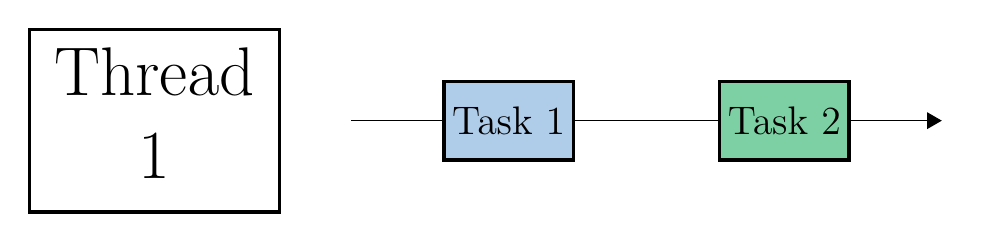
\begin{tikzpicture}
    
% 3. Draw connections manually or semi-automatically
\draw[-triangle 60]  (1,0) -- node[pos=1, anchor=west] {\textbf{\begin{tabular}{c} \end{tabular}}}(8.5,0);    
    % 1. Place the CPU
    \node[square] at (-1.5,0) {\begin{tabular}{c} Thread \\ 1 \end{tabular}};;

    % 2. Place Tasks using (X, Y) coordinates
    %    x = "Time start", y = "Lane height"
    \node[blue] (t1) at (3,0) {Task 1}; 
    \node[green] (t2) at (6.5,0) {Task 2}; 

%\node[scale=1.2] at (0.5,0) {\Huge \textbf{:}};

%\draw[-triangle 60]  (2.5,7) -- node[pos=1, anchor=west] {\textbf{\begin{tabular}{c} Definition \end{tabular}}}(3.6371,7);
%\draw[-triangle 60]  (2.5,6.5) -- node[pos=1, anchor=west] {\textbf{\begin{tabular}{c} Income and Price Changes \end{tabular}}}(3.6371,6.5);
% Vertical lines connecting arrows to text
%\draw (2.5,7) -- (2.5,6.5);

\end{tikzpicture}

\end{document}




